%!TEX root = ../main.tex
% file: assignment2.tex

\section{Assignment Two: Denoising of Signals} % (fold)
\label{sec:assignment_two_denoising_of_signals}

In this section we show the ability of the Fast Fourier Transform to filter signals in order to remove unwanted noise. Such denoising may be performed in multiple manners: high pass filtering, low pass filtering, and amplitude filtering. The FFT is applied to a sample wave file of a student's voice with natural background noise as well as added static of high and low amplitudes. We see that to remove background noise amplitude filtering is sufficient, however to remove static of various amplitudes, we must apply high and low pass filters.

\subsection{Method} % (fold)
\label{sub:method}
We begin by loading a sample wave file using the scipy \emph{wavfile} module.

\begin{lstlisting}[caption={Sound File Reading},label=lst:readsound,firstnumber=6]
    def readTone():
        from scipy.io import wavfile
        inFile = './static_noise_test.wav'
        tone = wavfile.read(inFile)
        return tone[1]
\end{lstlisting}
Listing \ref{lst:readsound} depicts the flow of loading the sound file. We first use \emph{wavfile} to read the file, however we only return the second row of the list, which contains our sound data.
\\\\
Once the sound data is stored in a numpy array, we then apply the real FFT to our sound data.
\begin{figure}[H]
    \centering
        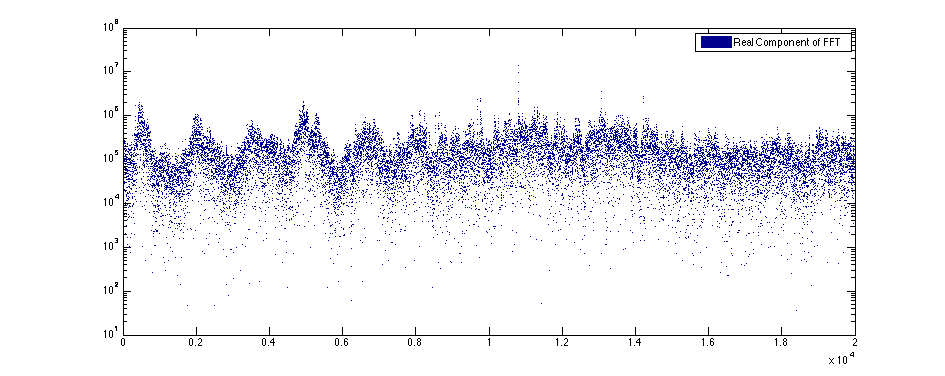
\includegraphics[width=6.5in]{./include/beforefig.png}
    \caption{Real Component of FFT Before Filtering}
    \label{fig:beforeFilt}
\end{figure}\noindent
Figure~\ref{fig:beforeFilt} depicts the real component of the signal spectrum once the FFT is applied. Note that there is also an imaginary component, however it is not plotted due to brevity. The plot is shown from 20Hz to 20kHz range which is approximately the range of human hearing. In order to isolate the voice in this signal, we assume that the frequency of the human voice occurs in the 200Hz to 10kHz range, and background noise carries low amplitude. We apply a total of three filters: a low pass filter, which removes high frequencies, a high pass filter, which removes low frequencies, and a amplitude filter, which removes frequencies of low amplitude.
\\\\
We begin by splitting the result of the FFT:
\begin{lstlisting}[caption={Splitting Spectrum into Real and Imaginary Components},label=lst:split,firstnumber=18]
    p = lambda z: (abs(real(z)),abs(imag(z)))
    temp = p(data)
\end{lstlisting}
Listing \ref{lst:split} splits the spectrum into real and imaginary components. This is done by applying the lambda function \emph{p}, then storing the result in a temporary array.
\\\\
We then apply a loop which filters the data.
\begin{lstlisting}[caption={Filter Application},label=lst:filter,firstnumber=21]
    for i in range(len(temp[0][:])):
        # amplitude filter in real
        if temp[0][i] <= ampfiltreal:
            data[i] = 0
        else:
            data[i] *= 10
        # amplitude filter in imaginary
        if temp[1][i] <= ampfiltimag:
            data[i] = 0
        # highpass filter in real and imaginary
        if i < highpass:
            data[i] = 0
        # lowpass filter in real and imaginary
        if i > lowpass:
            data[i] = 0
\end{lstlisting}
In Listing \ref{lst:filter} we see a total of four filters applied. We apply the amplitude filter to both real and imaginary components; the 'else' statement is there to amplify the isolated voice. The lowpass and highpass filters are not performed on amplitude, but rather on array position, which corresponds to frequency. 

\begin{figure}[H]
    \centering
        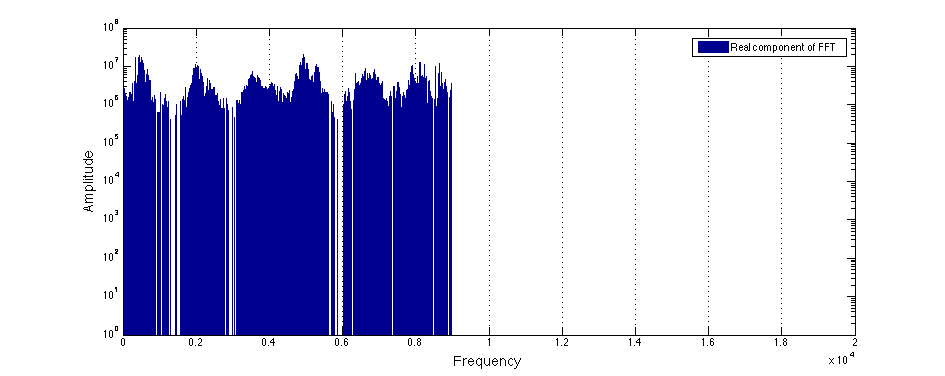
\includegraphics[width=6.5in]{./include/afterfig.png}
    \caption{Real Component of FFT After Filtering}
    \label{fig:afterFilt}
\end{figure}\noindent
Figure~\ref{fig:afterFilt} shows the resulting spectrum after applying filtering. The low pass filter is clearly evident as all frequencies above 10kHz are now zero. Due to the scaling of the plot, the high pass filter is not as clearly evident. The gaps shown in the plot of frequency correspond to amplitude filtered frequencies, or background noise.
\begin{lstlisting}[caption={Inverse Real FFT},label=lst:irfft,firstnumber=57]
    result = fft.irfft(F)
\end{lstlisting}
Now that filtering has been performed, we apply the inverse real FFT to reconstruct the sound signal.
% subsection method (end) 
\subsection{Results} % (fold)
\label{sub:results}
The result of this assignment may be heard in the sound files provided. File \emph{static\_noise\_test.wav} is the initial noisy sound file, whereas \emph{result.wav} is the filtered result. Let it be noted that there is additional noise introduced to the file which makes the voice sound muffled. It was found that the filtering of the FFT on such high amplitudes (such as voice), introduced oscillations into the time domain from the inverse FFT. In order to remedy these issues it would necessary to perform piecewise discontinuous smoothing to dampen the oscillations; this however exceeds the scope of the project.

% subsection results (end)

% section assignment_two_denoising_of_signals (end)